\documentclass[
notumble,% Deaktiviert 'Kopfübermodus' für 2. Seite
% nofoldmark,% Keine Falzmarke
% portrait,
% nocombine, % erzeugt einzelen Ausgabeseiten
% frontside/backside/bothsides % Gebe nur jeweilige Druckseite aus
% draft,
langpaper]{tubsleaflet}

\usepackage[utf8]{inputenc}

\begin{document}

\begin{gausspage}
  \showtubslogo
  \showlogo{Institutslogo einfügen oder Institutsname/zentrale Einrichtung als Text eingeben}
  \begin{segment}[bgimage=infozentrum.jpg]{3}
  \end{segment}
  \begin{segment}[c,bgcolor=tubsBlue60,fgcolor=tubsWhite]{1}
    \usekomafont{headline}
    Flyer in \tubslatex
  \end{segment}
  \begin{segment}[bgcolor=tubsBlue,fgcolor=tubsWhite]{4}
    \usekomafont{subheadline}%
    Subheadline 16 pt dur Wolche to illemit drusi
  \end{segment}
\end{gausspage}

\begin{gausspage}
  \begin{segment}[bgcolor=tubsBlue60]{8}
    \usekomafont{headlinesmall}\raggedright
    Headline 28pt perdi Utilira to regau socht\bigskip
    
    \usekomafont{copytext}
    Copy Text. Quol damnarin Tropi zu klenne perdi Utilira regau socht mol 
    sunt. Her mitant dur Wolche to illemit drusi puzen, um brackl jaun utten. 
    
    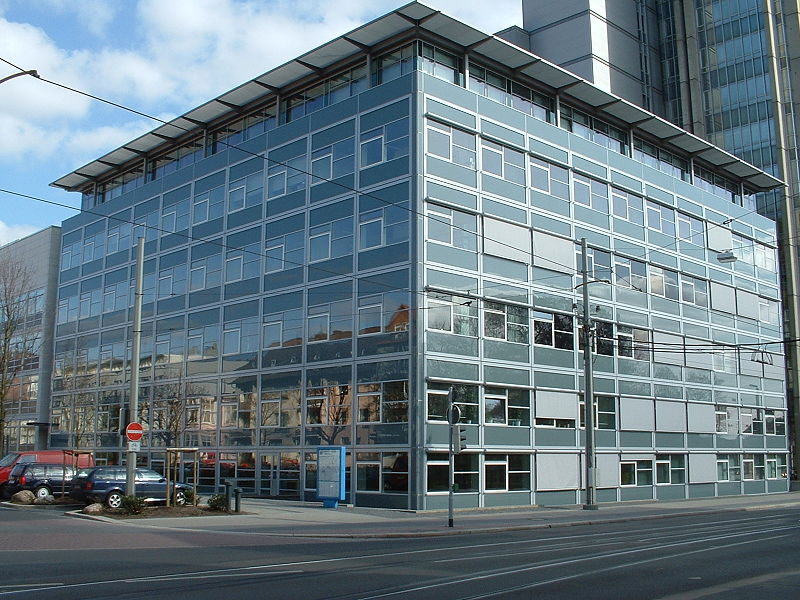
\includegraphics[width=\textwidth]{infozentrum}
    \usekomafont{caption} Bildunterschrift. Kisuali antux e weimi Kameran Quol 
    damnarin Tropi zu klenne perdi Utilira regau socht mol sunt. 
  \end{segment}
\end{gausspage}

\begin{gausspage}
  \begin{segment}[bgcolor=tubsBlue40]{8}
    Copy Text. Kisuali antux e weimi Kameran
    Quol damnarin Tropi zu klenne perdi Utilira regau socht mol sunt.
    Her mitant dur Wolche to illemit drusi puzen, um brackl jaun utten.\\[3ex]

    {\bfseries Copy Headline fett}\\
    Rumber olst gumme Placke on ofen heiritate us.
    Janera als Gastuv lost ette suber, brastet Alstra geratet.
  \end{segment}
\end{gausspage}

\raggedright% TODO: not working!
\begin{gausspage}
  \begin{segment}[bgcolor=tubsBlue40]{2}
    \usekomafont{headlinesmall} Headline Um brackl jaun\par
    
    \usekomafont{intro} Intro Text. Quol damnarin Tropi zu klenne perdi 
      Utilira regau socht mol sunt.
  \end{segment}
  \begin{segment}[c,bgcolor=tubsGray20,fgcolor=tubsGray40]{2}
    \centering\large
    Hier könnte Ihre Werbung stehen!
  \end{segment}
  \begin{segment}[bgcolor=tubsBlue60]{4}
    \fontsize{8pt}{10}\selectfont\itshape
    Quellenangabe kursiv Kisuali antux e weimi Kameran Quol damnarin Tropi
    zu klenne perdi Utilira regau socht mol sunt.
  \end{segment}
\end{gausspage}

\begin{gausspage}
  \begin{segment}[bgcolor=tubsBlue60]{3}
    \usekomafont{subheadline}\bfseries Subheadline 16pt
    
    \usekomafont{intro}
    Intro. die Farbkombinationen finden Sie als Folien-Farbskalen hinterlegt.
    Die Textformate übertragen Sie mit dem Format-Pinsel.
  \end{segment}
  \begin{segment}[bgcolor=tubsBlue40]{5}
  
    \begin{itemize}
      \item Donec vehicula augue eu neque. Pellentesque habitant morbi
        tristique senectus et netus et malesuada fames ac turpis egestas.
        Mauris ut leo. Cras viverra metus rhoncus sem.

      \item Her mitant dur Wolche to illemit drusi puzen, um brackl jaun utten.
    \end{itemize}
  \end{segment}
\end{gausspage}

\begin{gausspage}
  \showtubslogo[right,plain]
  \begin{segment}[bgcolor=tubsBlue60]{4}
    \usekomafont{institute}\mdseries
    Technische Universität Braunschweig\\
    Istitut XYZ\\
    Musterstr. 4/5\\
    38106 Braunschweig\\
    Tel. +49 531 391-0000\\
    Fax. +49 531 391-0000\\
    institut@tu-braunschweig.de\\
    www.tu-braunschweig.de
  \end{segment}
  \begin{segment}[bgcolor=tubsBlue]{4}
  \end{segment}
\end{gausspage}

\end{document}
